\tikzset{thick,every node/.style={scale=1}}
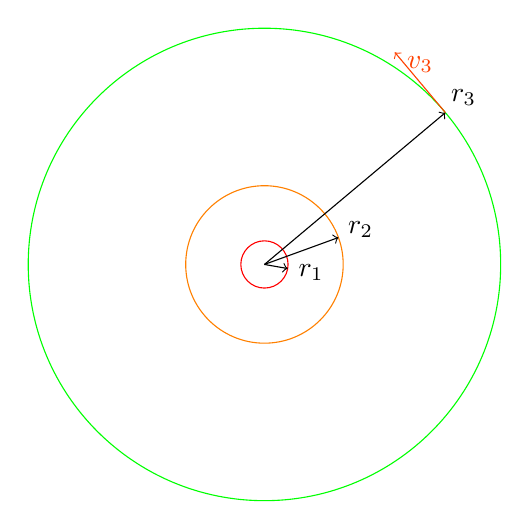
\begin{tikzpicture}
  \def\innCir{0.3};
  \def\outCir{3};
  \def\midCir{1};
  \def\innAng{-10};
  \def\midAng{20};
  \def\outAng{40};
  \def\lenVel{1};

  \draw[red] (0,0) circle(\innCir);
  \draw[orange] (0,0) circle(\midCir);
  \draw[green] (0,0) circle(\outCir);
  \draw[->] (0,0) to node[pos=2] {$r_1$} (\innAng:\innCir);
  \draw[->] (0,0) to node[pos=1.3] {$r_2$} (\midAng:\midCir);
  \draw[->] (0,0) to node[pos=1.1] {$r_3$} (\outAng:\outCir);
  \draw[->,red!50!orange] (\outAng:\outCir) to node[above] {$v_3$} ++(\outAng+90:\lenVel);
\end{tikzpicture}
